\chapter{We hear From Yanina}

If Valentine could have seen the trembling step and agitated
countenance of Franz when he quitted the chamber of M. Noirtier, even
she would have been constrained to pity him. Villefort had only just
given utterance to a few incoherent sentences, and then retired to his
study, where he received about two hours afterwards the following
letter:

\begin{quote}
{\small“After all the disclosures which were made this morning, M. Noirtier de
Villefort must see the utter impossibility of any alliance being formed
between his family and that of M. Franz d’Épinay. M. d’Épinay must say
that he is shocked and astonished that M. de Villefort, who appeared to
be aware of all the circumstances detailed this morning, should not
have anticipated him in this announcement.”}
\end{quote}

No one who had seen the magistrate at this moment, so thoroughly
unnerved by the recent inauspicious combination of circumstances, would
have supposed for an instant that he had anticipated the annoyance;
although it certainly never had occurred to him that his father would
carry candor, or rather rudeness, so far as to relate such a history.
And in justice to Villefort, it must be understood that M. Noirtier,
who never cared for the opinion of his son on any subject, had always
omitted to explain the affair to Villefort, so that he had all his life
entertained the belief that General de Quesnel, or the Baron d’Épinay,
as he was alternately styled, according as the speaker wished to
identify him by his own family name, or by the title which had been
conferred on him, fell the victim of assassination, and not that he was
killed fairly in a duel. This harsh letter, coming as it did from a man
generally so polite and respectful, struck a mortal blow at the pride
of Villefort.

Hardly had he read the letter, when his wife entered. The sudden
departure of Franz, after being summoned by M. Noirtier, had so much
astonished everyone, that the position of Madame de Villefort, left
alone with the notary and the witnesses, became every moment more
embarrassing. Determined to bear it no longer, she arose and left the
room; saying she would go and make some inquiries into the cause of his
sudden disappearance.

M. de Villefort’s communications on the subject were very limited and
concise; he told her, in fact, that an explanation had taken place
between M. Noirtier, M. d’Épinay, and himself, and that the marriage of
Valentine and Franz would consequently be broken off. This was an
awkward and unpleasant thing to have to report to those who were
waiting. She therefore contented herself with saying that M. Noirtier
having at the commencement of the discussion been attacked by a sort of
apoplectic fit, the affair would necessarily be deferred for some days
longer. This news, false as it was following so singularly in the train
of the two similar misfortunes which had so recently occurred,
evidently astonished the auditors, and they retired without a word.

During this time Valentine, at once terrified and happy, after having
embraced and thanked the feeble old man for thus breaking with a single
blow the chain which she had been accustomed to consider as
irrefragable, asked leave to retire to her own room, in order to
recover her composure. Noirtier looked the permission which she
solicited. But instead of going to her own room, Valentine, having once
gained her liberty, entered the gallery, and, opening a small door at
the end of it, found herself at once in the garden.

In the midst of all the strange events which had crowded one on the
other, an indefinable sentiment of dread had taken possession of
Valentine’s mind. She expected every moment that she should see Morrel
appear, pale and trembling, to forbid the signing of the contract, like
the Laird of Ravenswood in \textit{The Bride of Lammermoor}.

It was high time for her to make her appearance at the gate, for
Maximilian had long awaited her coming. He had half guessed what was
going on when he saw Franz quit the cemetery with M. de Villefort. He
followed M. d’Épinay, saw him enter, afterwards go out, and then
re-enter with Albert and Château-Renaud. He had no longer any doubts as
to the nature of the conference; he therefore quickly went to the gate
in the clover-patch, prepared to hear the result of the proceedings,
and very certain that Valentine would hasten to him the first moment
she should be set at liberty. He was not mistaken; peering through the
crevices of the wooden partition, he soon discovered the young girl,
who cast aside all her usual precautions and walked at once to the
barrier. The first glance which Maximilian directed towards her
entirely reassured him, and the first words she spoke made his heart
bound with delight.

“We are saved!” said Valentine.

“Saved?” repeated Morrel, not being able to conceive such intense
happiness; “by whom?”

“By my grandfather. Oh, Morrel, pray love him for all his goodness to
us!”

Morrel swore to love him with all his soul; and at that moment he could
safely promise to do so, for he felt as though it were not enough to
love him merely as a friend or even as a father, he worshiped him as a
god.

“But tell me, Valentine, how has it all been effected? What strange
means has he used to compass this blessed end?”

Valentine was on the point of relating all that had passed, but she
suddenly remembered that in doing so she must reveal a terrible secret
which concerned others as well as her grandfather, and she said:

“At some future time I will tell you all about it.”

“But when will that be?”

“When I am your wife.”

The conversation had now turned upon a topic so pleasing to Morrel,
that he was ready to accede to anything that Valentine thought fit to
propose, and he likewise felt that a piece of intelligence such as he
just heard ought to be more than sufficient to content him for one day.
However, he would not leave without the promise of seeing Valentine
again the next night. Valentine promised all that Morrel required of
her, and certainly it was less difficult now for her to believe that
she should marry Maximilian than it was an hour ago to assure herself
that she should not marry Franz.

During the time occupied by the interview we have just detailed, Madame
de Villefort had gone to visit M. Noirtier. The old man looked at her
with that stern and forbidding expression with which he was accustomed
to receive her.

“Sir,” said she, “it is superfluous for me to tell you that Valentine’s
marriage is broken off, since it was here that the affair was
concluded.”

Noirtier’s countenance remained immovable.

“But one thing I can tell you, of which I do not think you are aware;
that is, that I have always been opposed to this marriage, and that the
contract was entered into entirely without my consent or approbation.”

Noirtier regarded his daughter-in-law with the look of a man desiring
an explanation.

“Now that this marriage, which I know you so much disliked, is done
away with, I come to you on an errand which neither M. de Villefort nor
Valentine could consistently undertake.”

Noirtier’s eyes demanded the nature of her mission.

“I come to entreat you, sir,” continued Madame de Villefort, “as the
only one who has the right of doing so, inasmuch as I am the only one
who will receive no personal benefit from the transaction,—I come to
entreat you to restore, not your love, for that she has always
possessed, but to restore your fortune to your granddaughter.”

There was a doubtful expression in Noirtier’s eyes; he was evidently
trying to discover the motive of this proceeding, and he could not
succeed in doing so.

“May I hope, sir,” said Madame de Villefort, “that your intentions
accord with my request?”

Noirtier made a sign that they did.

“In that case, sir,” rejoined Madame de Villefort, “I will leave you
overwhelmed with gratitude and happiness at your prompt acquiescence to
my wishes.” She then bowed to M. Noirtier and retired.

The next day M. Noirtier sent for the notary; the first will was torn
up and a second made, in which he left the whole of his fortune to
Valentine, on condition that she should never be separated from him. It
was then generally reported that Mademoiselle de Villefort, the heiress
of the marquis and marchioness of Saint-Méran, had regained the good
graces of her grandfather, and that she would ultimately be in
possession of an income of 300,000 livres.

While all the proceedings relative to the dissolution of the
marriage-contract were being carried on at the house of M. de
Villefort, Monte Cristo had paid his visit to the Count of Morcerf,
who, in order to lose no time in responding to M. Danglars’ wishes, and
at the same time to pay all due deference to his position in society,
donned his uniform of lieutenant-general, which he ornamented with all
his crosses, and thus attired, ordered his finest horses and drove to
the Rue de la Chaussée d’Antin.

Danglars was balancing his monthly accounts, and it was perhaps not the
most favorable moment for finding him in his best humor. At the first
sight of his old friend, Danglars assumed his majestic air, and settled
himself in his easy-chair.

Morcerf, usually so stiff and formal, accosted the banker in an affable
and smiling manner, and, feeling sure that the overture he was about to
make would be well received, he did not consider it necessary to adopt
any manœuvres in order to gain his end, but went at once straight to
the point.

\begin{figure}[ht]
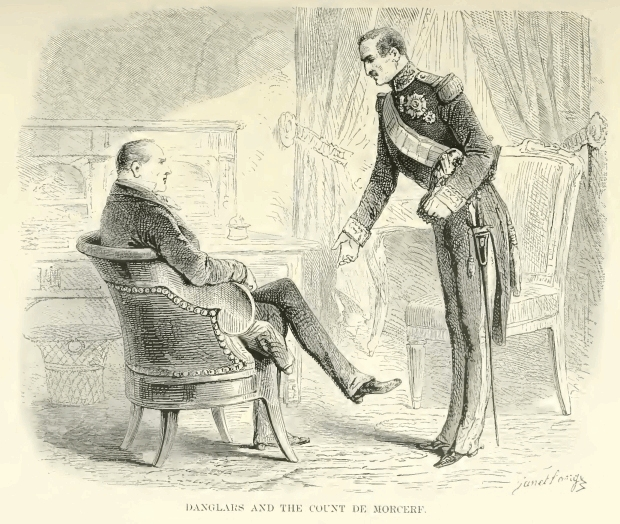
\includegraphics[width=\textwidth]{40086m.jpg}
\end{figure}

“Well, baron,” said he, “here I am at last; some time has elapsed since
our plans were formed, and they are not yet executed.”

Morcerf paused at these words, quietly waiting till the cloud should
have dispersed which had gathered on the brow of Danglars, and which he
attributed to his silence; but, on the contrary, to his great surprise,
it grew darker and darker.

“To what do you allude, monsieur?” said Danglars; as if he were trying
in vain to guess at the possible meaning of the general’s words.

“Ah,” said Morcerf, “I see you are a stickler for forms, my dear sir,
and you would remind me that the ceremonial rites should not be
omitted. \textit{Ma foi}, I beg your pardon, but as I have but one son, and it
is the first time I have ever thought of marrying him, I am still
serving my apprenticeship, you know; come, I will reform.”

And Morcerf with a forced smile arose, and, making a low bow to M.
Danglars, said:

“Baron, I have the honor of asking of you the hand of Mademoiselle
Eugénie Danglars for my son, the Vicomte Albert de Morcerf.”

But Danglars, instead of receiving this address in the favorable manner
which Morcerf had expected, knit his brow, and without inviting the
count, who was still standing, to take a seat, he said:

“Monsieur, it will be necessary to reflect before I give you an
answer.”

“To reflect?” said Morcerf, more and more astonished; “have you not had
enough time for reflection during the eight years which have elapsed
since this marriage was first discussed between us?”

“Count,” said the banker, “things are constantly occurring in the world
to induce us to lay aside our most established opinions, or at all
events to cause us to remodel them according to the change of
circumstances, which may have placed affairs in a totally different
light to that in which we at first viewed them.”

“I do not understand you, baron,” said Morcerf.

“What I mean to say is this, sir,—that during the last fortnight
unforeseen circumstances have occurred——”

“Excuse me,” said Morcerf, “but is it a play we are acting?”

“A play?”

“Yes, for it is like one; pray let us come more to the point, and
endeavor thoroughly to understand each other.”

“That is quite my desire.”

“You have seen M. de Monte Cristo have you not?”

“I see him very often,” said Danglars, drawing himself up; “he is a
particular friend of mine.”

“Well, in one of your late conversations with him, you said that I
appeared to be forgetful and irresolute concerning this marriage, did
you not?”

“I did say so.”

“Well, here I am, proving at once that I am really neither the one nor
the other, by entreating you to keep your promise on that score.”

Danglars did not answer.

“Have you so soon changed your mind,” added Morcerf, “or have you only
provoked my request that you may have the pleasure of seeing me
humbled?”

Danglars, seeing that if he continued the conversation in the same tone
in which he had begun it, the whole thing might turn out to his own
disadvantage, turned to Morcerf, and said:

“Count, you must doubtless be surprised at my reserve, and I assure you
it costs me much to act in such a manner towards you; but, believe me
when I say that imperative necessity has imposed the painful task upon
me.”

“These are all so many empty words, my dear sir,” said Morcerf: “they
might satisfy a new acquaintance, but the Comte de Morcerf does not
rank in that list; and when a man like him comes to another, recalls to
him his plighted word, and this man fails to redeem the pledge, he has
at least a right to exact from him a good reason for so doing.”

Danglars was a coward, but did not wish to appear so; he was piqued at
the tone which Morcerf had just assumed.

“I am not without a good reason for my conduct,” replied the banker.

“What do you mean to say?”

“I mean to say that I have a good reason, but that it is difficult to
explain.”

“You must be aware, at all events, that it is impossible for me to
understand motives before they are explained to me; but one thing at
least is clear, which is, that you decline allying yourself with my
family.”

“No, sir,” said Danglars; “I merely suspend my decision, that is all.”

“And do you really flatter yourself that I shall yield to all your
caprices, and quietly and humbly await the time of again being received
into your good graces?”

“Then, count, if you will not wait, we must look upon these projects as
if they had never been entertained.”

The count bit his lips till the blood almost started, to prevent the
ebullition of anger which his proud and irritable temper scarcely
allowed him to restrain; understanding, however, that in the present
state of things the laugh would decidedly be against him, he turned
from the door, towards which he had been directing his steps, and again
confronted the banker. A cloud settled on his brow, evincing decided
anxiety and uneasiness, instead of the expression of offended pride
which had lately reigned there.

“My dear Danglars,” said Morcerf, “we have been acquainted for many
years, and consequently we ought to make some allowance for each
other’s failings. You owe me an explanation, and really it is but fair
that I should know what circumstance has occurred to deprive my son of
your favor.”

“It is from no personal ill-feeling towards the viscount, that is all I
can say, sir,” replied Danglars, who resumed his insolent manner as
soon as he perceived that Morcerf was a little softened and calmed
down.

“And towards whom do you bear this personal ill-feeling, then?” said
Morcerf, turning pale with anger. The expression of the count’s face
had not remained unperceived by the banker; he fixed on him a look of
greater assurance than before, and said:

“You may, perhaps, be better satisfied that I should not go farther
into particulars.”

A tremor of suppressed rage shook the whole frame of the count, and
making a violent effort over himself, he said: “I have a right to
insist on your giving me an explanation. Is it Madame de Morcerf who
has displeased you? Is it my fortune which you find insufficient? Is it
because my opinions differ from yours?”

“Nothing of the kind, sir,” replied Danglars: “if such had been the
case, I only should have been to blame, inasmuch as I was aware of all
these things when I made the engagement. No, do not seek any longer to
discover the reason. I really am quite ashamed to have been the cause
of your undergoing such severe self-examination; let us drop the
subject, and adopt the middle course of delay, which implies neither a
rupture nor an engagement. \textit{Ma foi}, there is no hurry. My daughter is
only seventeen years old, and your son twenty-one. While we wait, time
will be progressing, events will succeed each other; things which in
the evening look dark and obscure, appear but too clearly in the light
of morning, and sometimes the utterance of one word, or the lapse of a
single day, will reveal the most cruel calumnies.”

“Calumnies, did you say, sir?” cried Morcerf, turning livid with rage.
“Does anyone dare to slander me?”

“Monsieur, I told you that I considered it best to avoid all
explanation.”

“Then, sir, I am patiently to submit to your refusal?”

“Yes, sir, although I assure you the refusal is as painful for me to
give as it is for you to receive, for I had reckoned on the honor of
your alliance, and the breaking off of a marriage contract always
injures the lady more than the gentleman.”

“Enough, sir,” said Morcerf, “we will speak no more on the subject.”

And clutching his gloves in anger, he left the apartment. Danglars
observed that during the whole conversation Morcerf had never once
dared to ask if it was on his own account that Danglars recalled his
word.

That evening he had a long conference with several friends; and M.
Cavalcanti, who had remained in the drawing-room with the ladies, was
the last to leave the banker’s house.

The next morning, as soon as he awoke, Danglars asked for the
newspapers; they were brought to him; he laid aside three or four, and
at last fixed on \textit{l’Impartial}, the paper of which Beauchamp was the
chief editor. He hastily tore off the cover, opened the journal with
nervous precipitation, passed contemptuously over the Paris jottings,
and arriving at the miscellaneous intelligence, stopped with a
malicious smile, at a paragraph headed

\begin{quote}
{\small\textit{We hear from Yanina.}}
\end{quote}

“Very good,” observed Danglars, after having read the paragraph; “here
is a little article on Colonel Fernand, which, if I am not mistaken,
would render the explanation which the Comte de Morcerf required of me
perfectly unnecessary.”

At the same moment, that is, at nine o’clock in the morning, Albert de
Morcerf, dressed in a black coat buttoned up to his chin, might have
been seen walking with a quick and agitated step in the direction of
Monte Cristo’s house in the Champs-Élysées. When he presented himself
at the gate the porter informed him that the Count had gone out about
half an hour previously.

“Did he take Baptistin with him?”

“No, my lord.”

“Call him, then; I wish to speak to him.”

The concierge went to seek the valet de chambre, and returned with him
in an instant.

“My good friend,” said Albert, “I beg pardon for my intrusion, but I
was anxious to know from your own mouth if your master was really out
or not.”

“He is really out, sir,” replied Baptistin.

“Out, even to me?”

“I know how happy my master always is to receive the vicomte,” said
Baptistin; “and I should therefore never think of including him in any
general order.”

“You are right; and now I wish to see him on an affair of great
importance. Do you think it will be long before he comes in?”

“No, I think not, for he ordered his breakfast at ten o’clock.”

“Well, I will go and take a turn in the Champs-Élysées, and at ten
o’clock I will return here; meanwhile, if the count should come in,
will you beg him not to go out again without seeing me?”

“You may depend on my doing so, sir,” said Baptistin.

Albert left the cab in which he had come at the count’s door, intending
to take a turn on foot. As he was passing the Allée des Veuves, he
thought he saw the count’s horses standing at Gosset’s
shooting-gallery; he approached, and soon recognized the coachman.

“Is the count shooting in the gallery?” said Morcerf.

“Yes, sir,” replied the coachman. While he was speaking, Albert had
heard the report of two or three pistol-shots. He entered, and on his
way met the waiter.

“Excuse me, my lord,” said the lad; “but will you have the kindness to
wait a moment?”

“What for, Philip?” asked Albert, who, being a constant visitor there,
did not understand this opposition to his entrance.

“Because the person who is now in the gallery prefers being alone, and
never practices in the presence of anyone.”

“Not even before you, Philip? Then who loads his pistol?”

“His servant.”

“A Nubian?”

“A negro.”

“It is he, then.”

“Do you know this gentleman?”

“Yes, and I am come to look for him; he is a friend of mine.”

“Oh, that is quite another thing, then. I will go immediately and
inform him of your arrival.”

And Philip, urged by his own curiosity, entered the gallery; a second
afterwards, Monte Cristo appeared on the threshold.

“I ask your pardon, my dear count,” said Albert, “for following you
here, and I must first tell you that it was not the fault of your
servants that I did so; I alone am to blame for the indiscretion. I
went to your house, and they told me you were out, but that they
expected you home at ten o’clock to breakfast. I was walking about in
order to pass away the time till ten o’clock, when I caught sight of
your carriage and horses.”

“What you have just said induces me to hope that you intend
breakfasting with me.”

\begin{figure}[ht]
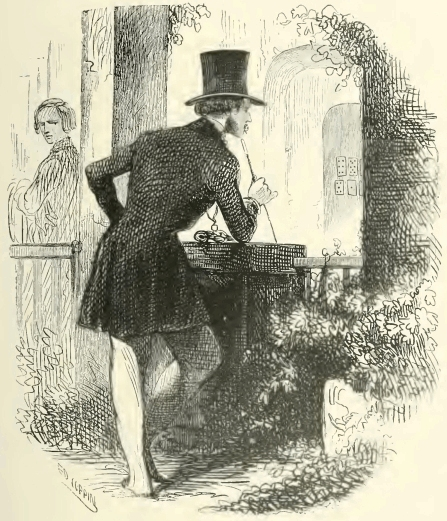
\includegraphics[width=\textwidth]{40092m.jpg}
\end{figure}

“No, thank you, I am thinking of other things besides breakfast just
now; perhaps we may take that meal at a later hour and in worse
company.”

“What on earth are you talking of?”

“I am to fight today.”

“For what?”

“For the sake of fighting!”

“Yes, I understand that, but what is the quarrel? People fight for all
sorts of reasons, you know.”

“I fight in the cause of honor.”

“Ah, that is something serious.”

“So serious, that I come to beg you to render me a service.”

“What is it?”

“To be my second.”

“That is a serious matter, and we will not discuss it here; let us
speak of nothing till we get home. Ali, bring me some water.”

The count turned up his sleeves, and passed into the little vestibule
where the gentlemen were accustomed to wash their hands after shooting.

“Come in, my lord,” said Philip in a low tone, “and I will show you
something droll.” Morcerf entered, and in place of the usual target, he
saw some playing-cards fixed against the wall. At a distance Albert
thought it was a complete suit, for he counted from the ace to the ten.

“Ah, ha,” said Albert, “I see you were preparing for a game of cards.”

“No,” said the count, “I was making a suit.”

“How?” said Albert.

“Those are really aces and twos which you see, but my shots have turned
them into threes, fives, sevens, eights, nines, and tens.”

Albert approached. In fact, the bullets had actually pierced the cards
in the exact places which the painted signs would otherwise have
occupied, the lines and distances being as regularly kept as if they
had been ruled with pencil. In going up to the target Morcerf picked up
two or three swallows that had been rash enough to come within the
range of the count’s pistol.

“\textit{Diable!}” said Morcerf.

“What would you have, my dear viscount?” said Monte Cristo, wiping his
hands on the towel which Ali had brought him; “I must occupy my leisure
moments in some way or other. But come, I am waiting for you.”

Both men entered Monte Cristo’s carriage, which in the course of a few
minutes deposited them safely at No. 30. Monte Cristo took Albert into
his study, and pointing to a seat, placed another for himself. “Now let
us talk the matter over quietly,” said the count.

“You see I am perfectly composed,” said Albert.

“With whom are you going to fight?”

“With Beauchamp.”

“One of your friends!”

“Of course; it is always with friends that one fights.”

“I suppose you have some cause of quarrel?”

“I have.”

\begin{figure}[ht]
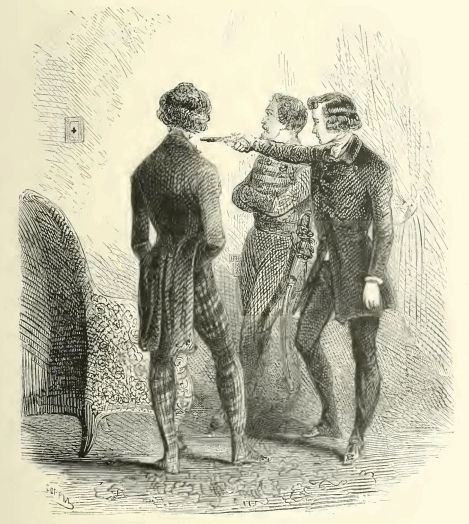
\includegraphics[width=\textwidth]{40094m.jpg}
\end{figure}

“What has he done to you?”

“There appeared in his journal last night—but wait, and read for
yourself.” And Albert handed over the paper to the count, who read as
follows:

\begin{quote}
{\small“A correspondent at Yanina informs us of a fact of which until now we
had remained in ignorance. The castle which formed the protection of
the town was given up to the Turks by a French officer named Fernand,
in whom the grand vizier, Ali Tepelini, had reposed the greatest
confidence.”}
\end{quote}

“Well,” said Monte Cristo, “what do you see in that to annoy you?”

“What do I see in it?”

“Yes; what does it signify to you if the castle of Yanina was given up
by a French officer?”

“It signifies to my father, the Count of Morcerf, whose Christian name
is Fernand!”

“Did your father serve under Ali Pasha?”

“Yes; that is to say, he fought for the independence of the Greeks, and
hence arises the calumny.”

“Oh, my dear viscount, do talk reason!”

“I do not desire to do otherwise.”

“Now, just tell me who the devil should know in France that the officer
Fernand and the Count of Morcerf are one and the same person? and who
cares now about Yanina, which was taken as long ago as the year 1822 or
1823?”

“That just shows the meanness of this slander. They have allowed all
this time to elapse, and then all of a sudden rake up events which have
been forgotten to furnish materials for scandal, in order to tarnish
the lustre of our high position. I inherit my father’s name, and I do
not choose that the shadow of disgrace should darken it. I am going to
Beauchamp, in whose journal this paragraph appears, and I shall insist
on his retracting the assertion before two witnesses.”

“Beauchamp will never retract.”

“Then we must fight.”

“No you will not, for he will tell you, what is very true, that perhaps
there were fifty officers in the Greek army bearing the same name.”

“We will fight, nevertheless. I will efface that blot on my father’s
character. My father, who was such a brave soldier, whose career was so
brilliant——”

“Oh, well, he will add, ‘We are warranted in believing that this
Fernand is not the illustrious Count of Morcerf, who also bears the
same Christian name.’”

“I am determined not to be content with anything short of an entire
retractation.”

“And you intend to make him do it in the presence of two witnesses, do
you?”

“Yes.”

“You do wrong.”

“Which means, I suppose, that you refuse the service which I asked of
you?”

“You know my theory regarding duels; I told you my opinion on that
subject, if you remember, when we were at Rome.”

“Nevertheless, my dear count, I found you this morning engaged in an
occupation but little consistent with the notions you profess to
entertain.”

“Because, my dear fellow, you understand one must never be eccentric.
If one’s lot is cast among fools, it is necessary to study folly. I
shall perhaps find myself one day called out by some harebrained scamp,
who has no more real cause of quarrel with me than you have with
Beauchamp; he may take me to task for some foolish trifle or other, he
will bring his witnesses, or will insult me in some public place, and I
am expected to kill him for all that.”

“You admit that you would fight, then? Well, if so, why do you object
to my doing so?”

“I do not say that you ought not to fight, I only say that a duel is a
serious thing, and ought not to be undertaken without due reflection.”

“Did he reflect before he insulted my father?”

“If he spoke hastily, and owns that he did so, you ought to be
satisfied.”

“Ah, my dear count, you are far too indulgent.”

“And you are far too exacting. Supposing, for instance, and do not be
angry at what I am going to say——”

“Well.”

“Supposing the assertion to be really true?”

“A son ought not to submit to such a stain on his father’s honor.”

“\textit{Ma foi!} we live in times when there is much to which we must
submit.”

“That is precisely the fault of the age.”

“And do you undertake to reform it?”

“Yes, as far as I am personally concerned.”

“Well, you are indeed exacting, my dear fellow!”

“Yes, I own it.”

“Are you quite impervious to good advice?”

“Not when it comes from a friend.”

“And do you account me that title?”

“Certainly I do.”

“Well, then, before going to Beauchamp with your witnesses, seek
further information on the subject.”

“From whom?”

“From Haydée.”

“Why, what can be the use of mixing a woman up in the affair?—what can
she do in it?”

“She can declare to you, for example, that your father had no hand
whatever in the defeat and death of the vizier; or if by chance he had,
indeed, the misfortune to——”

“I have told you, my dear count, that I would not for one moment admit
of such a proposition.”

“You reject this means of information, then?”

“I do—most decidedly.”

“Then let me offer one more word of advice.”

“Do so, then, but let it be the last.”

“You do not wish to hear it, perhaps?”

“On the contrary, I request it.”

“Do not take any witnesses with you when you go to Beauchamp—visit him
alone.”

“That would be contrary to all custom.”

“Your case is not an ordinary one.”

“And what is your reason for advising me to go alone?”

“Because then the affair will rest between you and Beauchamp.”

“Explain yourself.”

“I will do so. If Beauchamp be disposed to retract, you ought at least
to give him the opportunity of doing it of his own free will,—the
satisfaction to you will be the same. If, on the contrary, he refuses
to do so, it will then be quite time enough to admit two strangers into
your secret.”

“They will not be strangers, they will be friends.”

“Ah, but the friends of today are the enemies of tomorrow; Beauchamp,
for instance.”

“So you recommend——”

“I recommend you to be prudent.”

“Then you advise me to go alone to Beauchamp?”

“I do, and I will tell you why. When you wish to obtain some concession
from a man’s self-love, you must avoid even the appearance of wishing
to wound it.”

“I believe you are right.”

“I am glad of it.”

“Then I will go alone.”

“Go; but you would do better still by not going at all.”

“That is impossible.”

“Do so, then; it will be a wiser plan than the first which you
proposed.”

“But if, in spite of all my precautions, I am at last obliged to fight,
will you not be my second?”

“My dear viscount,” said Monte Cristo gravely, “you must have seen
before today that at all times and in all places I have been at your
disposal, but the service which you have just demanded of me is one
which it is out of my power to render you.”

“Why?”

“Perhaps you may know at some future period, and in the mean time I
request you to excuse my declining to put you in possession of my
reasons.”

“Well, I will have Franz and Château-Renaud; they will be the very men
for it.”

“Do so, then.”

“But if I do fight, you will surely not object to giving me a lesson or
two in shooting and fencing?”

“That, too, is impossible.”

“What a singular being you are!—you will not interfere in anything.”

“You are right—that is the principle on which I wish to act.”

“We will say no more about it, then. Good-bye, count.”

Morcerf took his hat, and left the room. He found his carriage at the
door, and doing his utmost to restrain his anger he went at once to
find Beauchamp, who was in his office. It was a gloomy, dusty-looking
apartment, such as journalists’ offices have always been from time
immemorial. The servant announced M. Albert de Morcerf. Beauchamp
repeated the name to himself, as though he could scarcely believe that
he had heard aright, and then gave orders for him to be admitted.
Albert entered.

Beauchamp uttered an exclamation of surprise on seeing his friend leap
over and trample under foot all the newspapers which were strewed about
the room.

“This way, this way, my dear Albert!” said he, holding out his hand to
the young man. “Are you out of your senses, or do you come peaceably to
take breakfast with me? Try and find a seat—there is one by that
geranium, which is the only thing in the room to remind me that there
are other leaves in the world besides leaves of paper.”

“Beauchamp,” said Albert, “it is of your journal that I come to speak.”

“Indeed? What do you wish to say about it?”

“I desire that a statement contained in it should be rectified.”

“To what do you refer? But pray sit down.”

“Thank you,” said Albert, with a cold and formal bow.

“Will you now have the kindness to explain the nature of the statement
which has displeased you?”

“An announcement has been made which implicates the honor of a member
of my family.”

“What is it?” said Beauchamp, much surprised; “surely you must be
mistaken.”

“The story sent you from Yanina.”

“Yanina?”

“Yes; really you appear to be totally ignorant of the cause which
brings me here.”

“Such is really the case, I assure you, upon my honor! Baptiste, give
me yesterday’s paper,” cried Beauchamp.

“Here, I have brought mine with me,” replied Albert.

Beauchamp took the paper, and read the article to which Albert pointed
in an undertone.

“You see it is a serious annoyance,” said Morcerf, when Beauchamp had
finished the perusal of the paragraph.

“Is the officer referred to a relation of yours, then?” demanded the
journalist.

“Yes,” said Albert, blushing.

“Well, what do you wish me to do for you?” said Beauchamp mildly.

“My dear Beauchamp, I wish you to contradict this statement.” Beauchamp
looked at Albert with a benevolent expression.

“Come,” said he, “this matter will want a good deal of talking over; a
retractation is always a serious thing, you know. Sit down, and I will
read it again.”

Albert resumed his seat, and Beauchamp read, with more attention than
at first, the lines denounced by his friend.

“Well,” said Albert in a determined tone, “you see that your paper has
insulted a member of my family, and I insist on a retractation being
made.”

“You insist?”

“Yes, I insist.”

“Permit me to remind you that you are not in the Chamber, my dear
viscount.”

“Nor do I wish to be there,” replied the young man, rising. “I repeat
that I am determined to have the announcement of yesterday
contradicted. You have known me long enough,” continued Albert, biting
his lips convulsively, for he saw that Beauchamp’s anger was beginning
to rise,—“you have been my friend, and therefore sufficiently intimate
with me to be aware that I am likely to maintain my resolution on this
point.”

“If I have been your friend, Morcerf, your present manner of speaking
would almost lead me to forget that I ever bore that title. But wait a
moment, do not let us get angry, or at least not yet. You are irritated
and vexed—tell me how this Fernand is related to you?”

“He is merely my father,” said Albert—“M. Fernand Mondego, Count of
Morcerf, an old soldier who has fought in twenty battles and whose
honorable scars they would denounce as badges of disgrace.”

“Is it your father?” said Beauchamp; “that is quite another thing. Then
I can well understand your indignation, my dear Albert. I will look at
it again;” and he read the paragraph for the third time, laying a
stress on each word as he proceeded. “But the paper nowhere identifies
this Fernand with your father.”

\begin{figure}[ht]
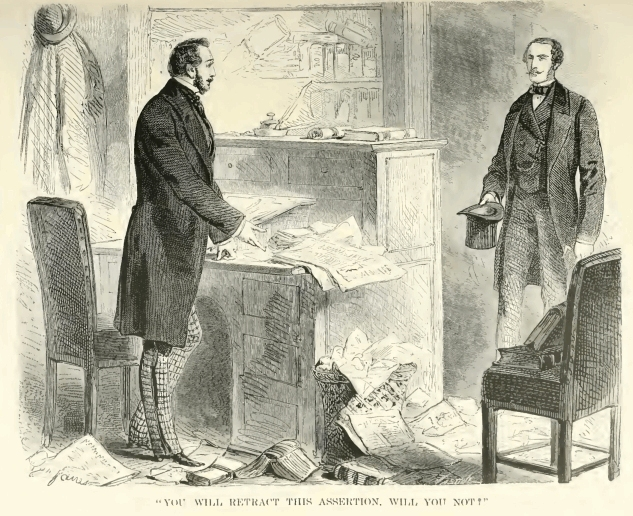
\includegraphics[width=\textwidth]{40100m.jpg}
\end{figure}

“No; but the connection will be seen by others, and therefore I will
have the article contradicted.”

At the words \textit{I will}, Beauchamp steadily raised his eyes to Albert’s
countenance, and then as gradually lowering them, he remained
thoughtful for a few moments.

“You will retract this assertion, will you not, Beauchamp?” said Albert
with increased though stifled anger.

“Yes,” replied Beauchamp.

“Immediately?” said Albert.

“When I am convinced that the statement is false.”

“What?”

“The thing is worth looking into, and I will take pains to investigate
the matter thoroughly.”

“But what is there to investigate, sir?” said Albert, enraged beyond
measure at Beauchamp’s last remark. “If you do not believe that it is
my father, say so immediately; and if, on the contrary, you believe it
to be him, state your reasons for doing so.”

Beauchamp looked at Albert with the smile which was so peculiar to him,
and which in its numerous modifications served to express every varied
emotion of his mind.

“Sir,” replied he, “if you came to me with the idea of demanding
satisfaction, you should have gone at once to the point, and not have
entertained me with the idle conversation to which I have been
patiently listening for the last half hour. Am I to put this
construction on your visit?”

“Yes, if you will not consent to retract that infamous calumny.”

“Wait a moment—no threats, if you please, M. Fernand Mondego, Vicomte
de Morcerf; I never allow them from my enemies, and therefore shall not
put up with them from my friends. You insist on my contradicting the
article relating to General Fernand, an article with which, I assure
you on my word of honor, I had nothing whatever to do?”

“Yes, I insist on it,” said Albert, whose mind was beginning to get
bewildered with the excitement of his feelings.

“And if I refuse to retract, you wish to fight, do you?” said Beauchamp
in a calm tone.

“Yes,” replied Albert, raising his voice.

“Well,” said Beauchamp, “here is my answer, my dear sir. The article
was not inserted by me—I was not even aware of it; but you have, by the
step you have taken, called my attention to the paragraph in question,
and it will remain until it shall be either contradicted or confirmed
by someone who has a right to do so.”

“Sir,” said Albert, rising, “I will do myself the honor of sending my
seconds to you, and you will be kind enough to arrange with them the
place of meeting and the weapons.”

“Certainly, my dear sir.”

“And this evening, if you please, or tomorrow at the latest, we will
meet.”

“No, no, I will be on the ground at the proper time; but in my opinion
(and I have a right to dictate the preliminaries, as it is I who have
received the provocation)—in my opinion the time ought not to be yet. I
know you to be well skilled in the management of the sword, while I am
only moderately so; I know, too, that you are a good marksman—there we
are about equal. I know that a duel between us two would be a serious
affair, because you are brave, and I am brave also. I do not therefore
wish either to kill you, or to be killed myself without a cause. Now, I
am going to put a question to you, and one very much to the purpose
too. Do you insist on this retractation so far as to kill me if I do
not make it, although I have repeated more than once, and affirmed on
my honor, that I was ignorant of the thing with which you charge me,
and although I still declare that it is impossible for anyone but you
to recognize the Count of Morcerf under the name of Fernand?”

“I maintain my original resolution.”

“Very well, my dear sir; then I consent to cut throats with you. But I
require three weeks’ preparation; at the end of that time I shall come
and say to you, ‘The assertion is false, and I retract it,’ or ‘The
assertion is true,’ when I shall immediately draw the sword from its
sheath, or the pistols from the case, whichever you please.”

“Three weeks!” cried Albert; “they will pass as slowly as three
centuries when I am all the time suffering dishonor.”

“Had you continued to remain on amicable terms with me, I should have
said, ‘Patience, my friend;’ but you have constituted yourself my
enemy, therefore I say, ‘What does that signify to me, sir?’”

“Well, let it be three weeks then,” said Morcerf; “but remember, at the
expiration of that time no delay or subterfuge will justify you in——”

“M. Albert de Morcerf,” said Beauchamp, rising in his turn, “I cannot
throw you out of window for three weeks—that is to say, for twenty-four
days to come—nor have you any right to split my skull open till that
time has elapsed. Today is the 29th of August; the 21st of September
will, therefore, be the conclusion of the term agreed on, and till that
time arrives—and it is the advice of a gentleman which I am about to
give you—till then we will refrain from growling and barking like two
dogs chained within sight of each other.”

When he had concluded his speech, Beauchamp bowed coldly to Albert,
turned his back upon him, and went to the press-room. Albert vented his
anger on a pile of newspapers, which he sent flying all over the office
by switching them violently with his stick; after which ebullition he
departed—not, however, without walking several times to the door of the
press-room, as if he had half a mind to enter.

\begin{figure}[ht]
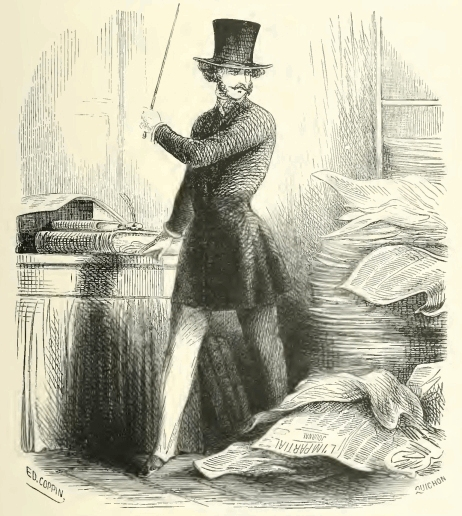
\includegraphics[width=\textwidth]{40104m.jpg}
\end{figure}

While Albert was lashing the front of his carriage in the same manner
that he had the newspapers which were the innocent agents of his
discomfiture, as he was crossing the barrier he perceived Morrel, who
was walking with a quick step and a bright eye. He was passing the
Chinese Baths, and appeared to have come from the direction of the
Porte Saint-Martin, and to be going towards the Madeleine.

“Ah,” said Morcerf, “there goes a happy man!” And it so happened Albert
was not mistaken in his opinion.
